% Options for packages loaded elsewhere
\PassOptionsToPackage{unicode}{hyperref}
\PassOptionsToPackage{hyphens}{url}
\documentclass[
]{book}
\usepackage{xcolor}
\usepackage{amsmath,amssymb}
\setcounter{secnumdepth}{5}
\usepackage{iftex}
\ifPDFTeX
  \usepackage[T1]{fontenc}
  \usepackage[utf8]{inputenc}
  \usepackage{textcomp} % provide euro and other symbols
\else % if luatex or xetex
  \usepackage{unicode-math} % this also loads fontspec
  \defaultfontfeatures{Scale=MatchLowercase}
  \defaultfontfeatures[\rmfamily]{Ligatures=TeX,Scale=1}
\fi
\usepackage{lmodern}
\ifPDFTeX\else
  % xetex/luatex font selection
\fi
% Use upquote if available, for straight quotes in verbatim environments
\IfFileExists{upquote.sty}{\usepackage{upquote}}{}
\IfFileExists{microtype.sty}{% use microtype if available
  \usepackage[]{microtype}
  \UseMicrotypeSet[protrusion]{basicmath} % disable protrusion for tt fonts
}{}
\makeatletter
\@ifundefined{KOMAClassName}{% if non-KOMA class
  \IfFileExists{parskip.sty}{%
    \usepackage{parskip}
  }{% else
    \setlength{\parindent}{0pt}
    \setlength{\parskip}{6pt plus 2pt minus 1pt}}
}{% if KOMA class
  \KOMAoptions{parskip=half}}
\makeatother
\usepackage{color}
\usepackage{fancyvrb}
\newcommand{\VerbBar}{|}
\newcommand{\VERB}{\Verb[commandchars=\\\{\}]}
\DefineVerbatimEnvironment{Highlighting}{Verbatim}{commandchars=\\\{\}}
% Add ',fontsize=\small' for more characters per line
\usepackage{framed}
\definecolor{shadecolor}{RGB}{248,248,248}
\newenvironment{Shaded}{\begin{snugshade}}{\end{snugshade}}
\newcommand{\AlertTok}[1]{\textcolor[rgb]{0.94,0.16,0.16}{#1}}
\newcommand{\AnnotationTok}[1]{\textcolor[rgb]{0.56,0.35,0.01}{\textbf{\textit{#1}}}}
\newcommand{\AttributeTok}[1]{\textcolor[rgb]{0.13,0.29,0.53}{#1}}
\newcommand{\BaseNTok}[1]{\textcolor[rgb]{0.00,0.00,0.81}{#1}}
\newcommand{\BuiltInTok}[1]{#1}
\newcommand{\CharTok}[1]{\textcolor[rgb]{0.31,0.60,0.02}{#1}}
\newcommand{\CommentTok}[1]{\textcolor[rgb]{0.56,0.35,0.01}{\textit{#1}}}
\newcommand{\CommentVarTok}[1]{\textcolor[rgb]{0.56,0.35,0.01}{\textbf{\textit{#1}}}}
\newcommand{\ConstantTok}[1]{\textcolor[rgb]{0.56,0.35,0.01}{#1}}
\newcommand{\ControlFlowTok}[1]{\textcolor[rgb]{0.13,0.29,0.53}{\textbf{#1}}}
\newcommand{\DataTypeTok}[1]{\textcolor[rgb]{0.13,0.29,0.53}{#1}}
\newcommand{\DecValTok}[1]{\textcolor[rgb]{0.00,0.00,0.81}{#1}}
\newcommand{\DocumentationTok}[1]{\textcolor[rgb]{0.56,0.35,0.01}{\textbf{\textit{#1}}}}
\newcommand{\ErrorTok}[1]{\textcolor[rgb]{0.64,0.00,0.00}{\textbf{#1}}}
\newcommand{\ExtensionTok}[1]{#1}
\newcommand{\FloatTok}[1]{\textcolor[rgb]{0.00,0.00,0.81}{#1}}
\newcommand{\FunctionTok}[1]{\textcolor[rgb]{0.13,0.29,0.53}{\textbf{#1}}}
\newcommand{\ImportTok}[1]{#1}
\newcommand{\InformationTok}[1]{\textcolor[rgb]{0.56,0.35,0.01}{\textbf{\textit{#1}}}}
\newcommand{\KeywordTok}[1]{\textcolor[rgb]{0.13,0.29,0.53}{\textbf{#1}}}
\newcommand{\NormalTok}[1]{#1}
\newcommand{\OperatorTok}[1]{\textcolor[rgb]{0.81,0.36,0.00}{\textbf{#1}}}
\newcommand{\OtherTok}[1]{\textcolor[rgb]{0.56,0.35,0.01}{#1}}
\newcommand{\PreprocessorTok}[1]{\textcolor[rgb]{0.56,0.35,0.01}{\textit{#1}}}
\newcommand{\RegionMarkerTok}[1]{#1}
\newcommand{\SpecialCharTok}[1]{\textcolor[rgb]{0.81,0.36,0.00}{\textbf{#1}}}
\newcommand{\SpecialStringTok}[1]{\textcolor[rgb]{0.31,0.60,0.02}{#1}}
\newcommand{\StringTok}[1]{\textcolor[rgb]{0.31,0.60,0.02}{#1}}
\newcommand{\VariableTok}[1]{\textcolor[rgb]{0.00,0.00,0.00}{#1}}
\newcommand{\VerbatimStringTok}[1]{\textcolor[rgb]{0.31,0.60,0.02}{#1}}
\newcommand{\WarningTok}[1]{\textcolor[rgb]{0.56,0.35,0.01}{\textbf{\textit{#1}}}}
\usepackage{longtable,booktabs,array}
\usepackage{calc} % for calculating minipage widths
% Correct order of tables after \paragraph or \subparagraph
\usepackage{etoolbox}
\makeatletter
\patchcmd\longtable{\par}{\if@noskipsec\mbox{}\fi\par}{}{}
\makeatother
% Allow footnotes in longtable head/foot
\IfFileExists{footnotehyper.sty}{\usepackage{footnotehyper}}{\usepackage{footnote}}
\makesavenoteenv{longtable}
\usepackage{graphicx}
\makeatletter
\newsavebox\pandoc@box
\newcommand*\pandocbounded[1]{% scales image to fit in text height/width
  \sbox\pandoc@box{#1}%
  \Gscale@div\@tempa{\textheight}{\dimexpr\ht\pandoc@box+\dp\pandoc@box\relax}%
  \Gscale@div\@tempb{\linewidth}{\wd\pandoc@box}%
  \ifdim\@tempb\p@<\@tempa\p@\let\@tempa\@tempb\fi% select the smaller of both
  \ifdim\@tempa\p@<\p@\scalebox{\@tempa}{\usebox\pandoc@box}%
  \else\usebox{\pandoc@box}%
  \fi%
}
% Set default figure placement to htbp
\def\fps@figure{htbp}
\makeatother
\setlength{\emergencystretch}{3em} % prevent overfull lines
\providecommand{\tightlist}{%
  \setlength{\itemsep}{0pt}\setlength{\parskip}{0pt}}
\usepackage[]{natbib}
\bibliographystyle{plainnat}
\usepackage{booktabs}
\usepackage{bookmark}
\IfFileExists{xurl.sty}{\usepackage{xurl}}{} % add URL line breaks if available
\urlstyle{same}
\hypersetup{
  pdftitle={Week 1: Econ 645 Introduction},
  pdfauthor={Samuel Rowe},
  hidelinks,
  pdfcreator={LaTeX via pandoc}}

\title{Week 1: Econ 645 Introduction}
\author{Samuel Rowe}
\date{2025-08-10}

\begin{document}
\maketitle

{
\setcounter{tocdepth}{1}
\tableofcontents
}
\chapter{Overview}\label{overview}

Welcome to Econ 645. We will cover how to implement Stata commands for econometrics, along with data management. Data management will be key for transparent and reproducible work or research. For tonight, we will cover the following topics before delving into Mitchell and Wooldridge:

\begin{itemize}
\tightlist
\item
  Julian Reif's Coding Guide Folder Structure
\item
  Executing do-files and making log files
\item
  Automate Graphs
\item
  Helpful Advanced Techniques
\item
  Publish your results
\end{itemize}

\chapter{Coding Guide for Folder Structure}\label{coding-guide-for-folder-structure}

Please see Julian Reif's coding guide at \url{https://julianreif.com/guide/}. These are very good tips very about repliciability and organization. Having your files organized in a folder as an example below will not only with organization, but with replication, as well. You can hand over the entire folder structure, and another users will be able to run the master do file with just changing the main folder location once.

Folder Structure

\begin{itemize}
\tightlist
\item
  ├── analysis/

  \begin{itemize}
  \tightlist
  \item
    ├── data/
  \item
    ├── processed/
  \item
    ├── results/

    \begin{itemize}
    \tightlist
    \item
      ├── figures/
    \item
      ├── tables/
    \item
      ├── scripts/

      \begin{itemize}
      \tightlist
      \item
        ├── 1\_process\_raw\_data.do
      \item
        ├── 2\_\ldots{}
      \end{itemize}
    \end{itemize}
  \item
    ├── run.do
  \end{itemize}
\item
  ├── paper/

  \begin{itemize}
  \tightlist
  \item
    ├── manuscript.tex
  \item
    ├── figures/
  \item
    ├── tables/
  \end{itemize}
\end{itemize}

\chapter{Executing do-files and making log files}\label{executing-do-files-and-making-log-files}

From Mitchell 10.3, you should always use a do file when you work with Stata. I find log files helpful, but do files are essential. Do files provide transparency to show your work, and it help provide replication. One key feature of do files are comments. Comments are an essential part for two reasons. It will help yourself when you go back to your own code to describe what is going one. Second, it helps
with replication, since someone should be able to run your code top to bottom and get the same results that you have in your paper, report, or document.

\emph{Never} use point and click. It is available in Stata, but don't lower yourself to a SPSS standard.

In case you are new to do files. We'll start off with a simple example. We'll pull some data, summarize some data, and tabulate some data.

\begin{Shaded}
\begin{Highlighting}[]
\KeywordTok{use}\NormalTok{ wws.dta, }\KeywordTok{clear}
\KeywordTok{summarize}\NormalTok{ age wage hours}
\KeywordTok{tabulate}\NormalTok{ married}
\end{Highlighting}
\end{Shaded}

\begin{verbatim}
/Users/Sam/Desktop/Econ 645/Data/Mitchell

(Working Women Survey)

    Variable |        Obs        Mean    Std. Dev.       Min        Max
-------------+---------------------------------------------------------
         age |      2,246    36.25111    5.437983         21         83
        wage |      2,246    288.2885    9595.692          0     380000
       hours |      2,242    37.21811    10.50914          1         80

    married |      Freq.     Percent        Cum.
------------+-----------------------------------
          0 |        804       35.80       35.80
          1 |      1,442       64.20      100.00
------------+-----------------------------------
      Total |      2,246      100.00
\end{verbatim}

We can look at a similar file called example1.do

\begin{Shaded}
\begin{Highlighting}[]
    \DecValTok{type}\NormalTok{ example1.}\KeywordTok{do}
\end{Highlighting}
\end{Shaded}

We can actually run a do file within a do file

\begin{Shaded}
\begin{Highlighting}[]
\KeywordTok{do}\NormalTok{ example1.}\KeywordTok{do}
\end{Highlighting}
\end{Shaded}

\begin{verbatim}
(Working Women Survey w/fixes)

    Variable |        Obs        Mean    Std. Dev.       Min        Max
-------------+---------------------------------------------------------
         age |      2,246    36.22707    5.337859         21         48
        wage |      2,244    7.796781     5.82459          0   40.74659
       hours |      2,242    37.21811    10.50914          1         80

    married |      Freq.     Percent        Cum.
------------+-----------------------------------
          0 |        804       35.80       35.80
          1 |      1,442       64.20      100.00
------------+-----------------------------------
      Total |      2,246      100.00
\end{verbatim}

You can use the doedit command if you want to open the Do-file Editor, but you can just click to open the Do-File (this is an exception from what I said above).

Since we already have the Do-File Editor open, running the doedit will just open a new blank do file.

\begin{Shaded}
\begin{Highlighting}[]
\NormalTok{doedit }
\end{Highlighting}
\end{Shaded}

Note: you can write do files in Notepad or TextEdit, but you don't get any
of the benefits, such as highlighted text.

Let's look at a do file that uses the log command

\begin{Shaded}
\begin{Highlighting}[]
\DecValTok{type}\NormalTok{ example2.}\KeywordTok{do}
\end{Highlighting}
\end{Shaded}

Let's run it.

\begin{Shaded}
\begin{Highlighting}[]
\FunctionTok{log} \KeywordTok{using}\NormalTok{ example2}
\KeywordTok{use}\NormalTok{ wws2, }\KeywordTok{clear}
\KeywordTok{summarize}\NormalTok{ age wage hours}
\KeywordTok{tabulate}\NormalTok{ married}
\FunctionTok{log} \KeywordTok{close}\NormalTok{ example2}
\end{Highlighting}
\end{Shaded}

\emph{Note:} It is important to note that when opening a log it must end with a ``log close'' command. If your do files bombs out (fails to finish) before reaching the log close command, your log will remain open.

Even if we close the log file, we'll get an error if we try to run the do file again. So we need to add the replace option.

\begin{Shaded}
\begin{Highlighting}[]
\FunctionTok{log} \KeywordTok{using}\NormalTok{ example2, }\KeywordTok{replace}
\KeywordTok{use}\NormalTok{ wws2, }\KeywordTok{clear}
\KeywordTok{summarize}\NormalTok{ age wage hours}
\KeywordTok{tabulate}\NormalTok{ married}
\FunctionTok{log} \KeywordTok{close}
\end{Highlighting}
\end{Shaded}

\begin{verbatim}
      name:  <unnamed>
       log:  /Users/Sam/Desktop/Econ 645/Data/Mitchell/example2.smcl
  log type:  smcl
 opened on:  10 Aug 2025, 09:41:12

(Working Women Survey w/fixes)

    Variable |        Obs        Mean    Std. Dev.       Min        Max
-------------+---------------------------------------------------------
         age |      2,246    36.22707    5.337859         21         48
        wage |      2,244    7.796781     5.82459          0   40.74659
       hours |      2,242    37.21811    10.50914          1         80

    married |      Freq.     Percent        Cum.
------------+-----------------------------------
          0 |        804       35.80       35.80
          1 |      1,442       64.20      100.00
------------+-----------------------------------
      Total |      2,246      100.00

      name:  <unnamed>
       log:  /Users/Sam/Desktop/Econ 645/Data/Mitchell/example2.smcl
  log type:  smcl
 closed on:  10 Aug 2025, 09:41:12
------------------------------------------------------------------------------------------------------------------
\end{verbatim}

\chapter{Automate Graphs and Figures}\label{automate-graphs-and-figures}

Stata makes saving graphs easy, so if there is a minor fix all you need to do is rerun the scripts and have your graph fixed. Use the \textbf{graph export} command to save a graph.

\begin{Shaded}
\begin{Highlighting}[]
\NormalTok{*Get CPS Data}
\KeywordTok{use}\NormalTok{ jun25pub.dta}
\KeywordTok{gen}\NormalTok{ earnings=pternwa/100 }\KeywordTok{if}\NormalTok{ prerelg==1}
\KeywordTok{histogram}\NormalTok{ earnings }\KeywordTok{if}\NormalTok{ prerelg==1, }\BaseNTok{title}\NormalTok{(}\StringTok{"Wages in June 2025"}\NormalTok{) }\BaseNTok{caption}\NormalTok{(}\StringTok{"Source: Current Population Survey"}\NormalTok{)}
\KeywordTok{graph} \KeywordTok{export} \StringTok{"Wages\_June\_2025.png"}
\end{Highlighting}
\end{Shaded}

\begin{verbatim}
/Users/Sam/Desktop/Econ 645/Data/CPS


(28,617 missing values generated)

    Variable |        Obs        Mean    Std. Dev.       Min        Max
-------------+---------------------------------------------------------
    earnings |      9,939    1596.086    2184.658          0   13145.81

(bin=39, start=0, width=337.07205)
option replace not allowed
r(198);

r(198);
\end{verbatim}

\begin{figure}
\centering
\pandocbounded{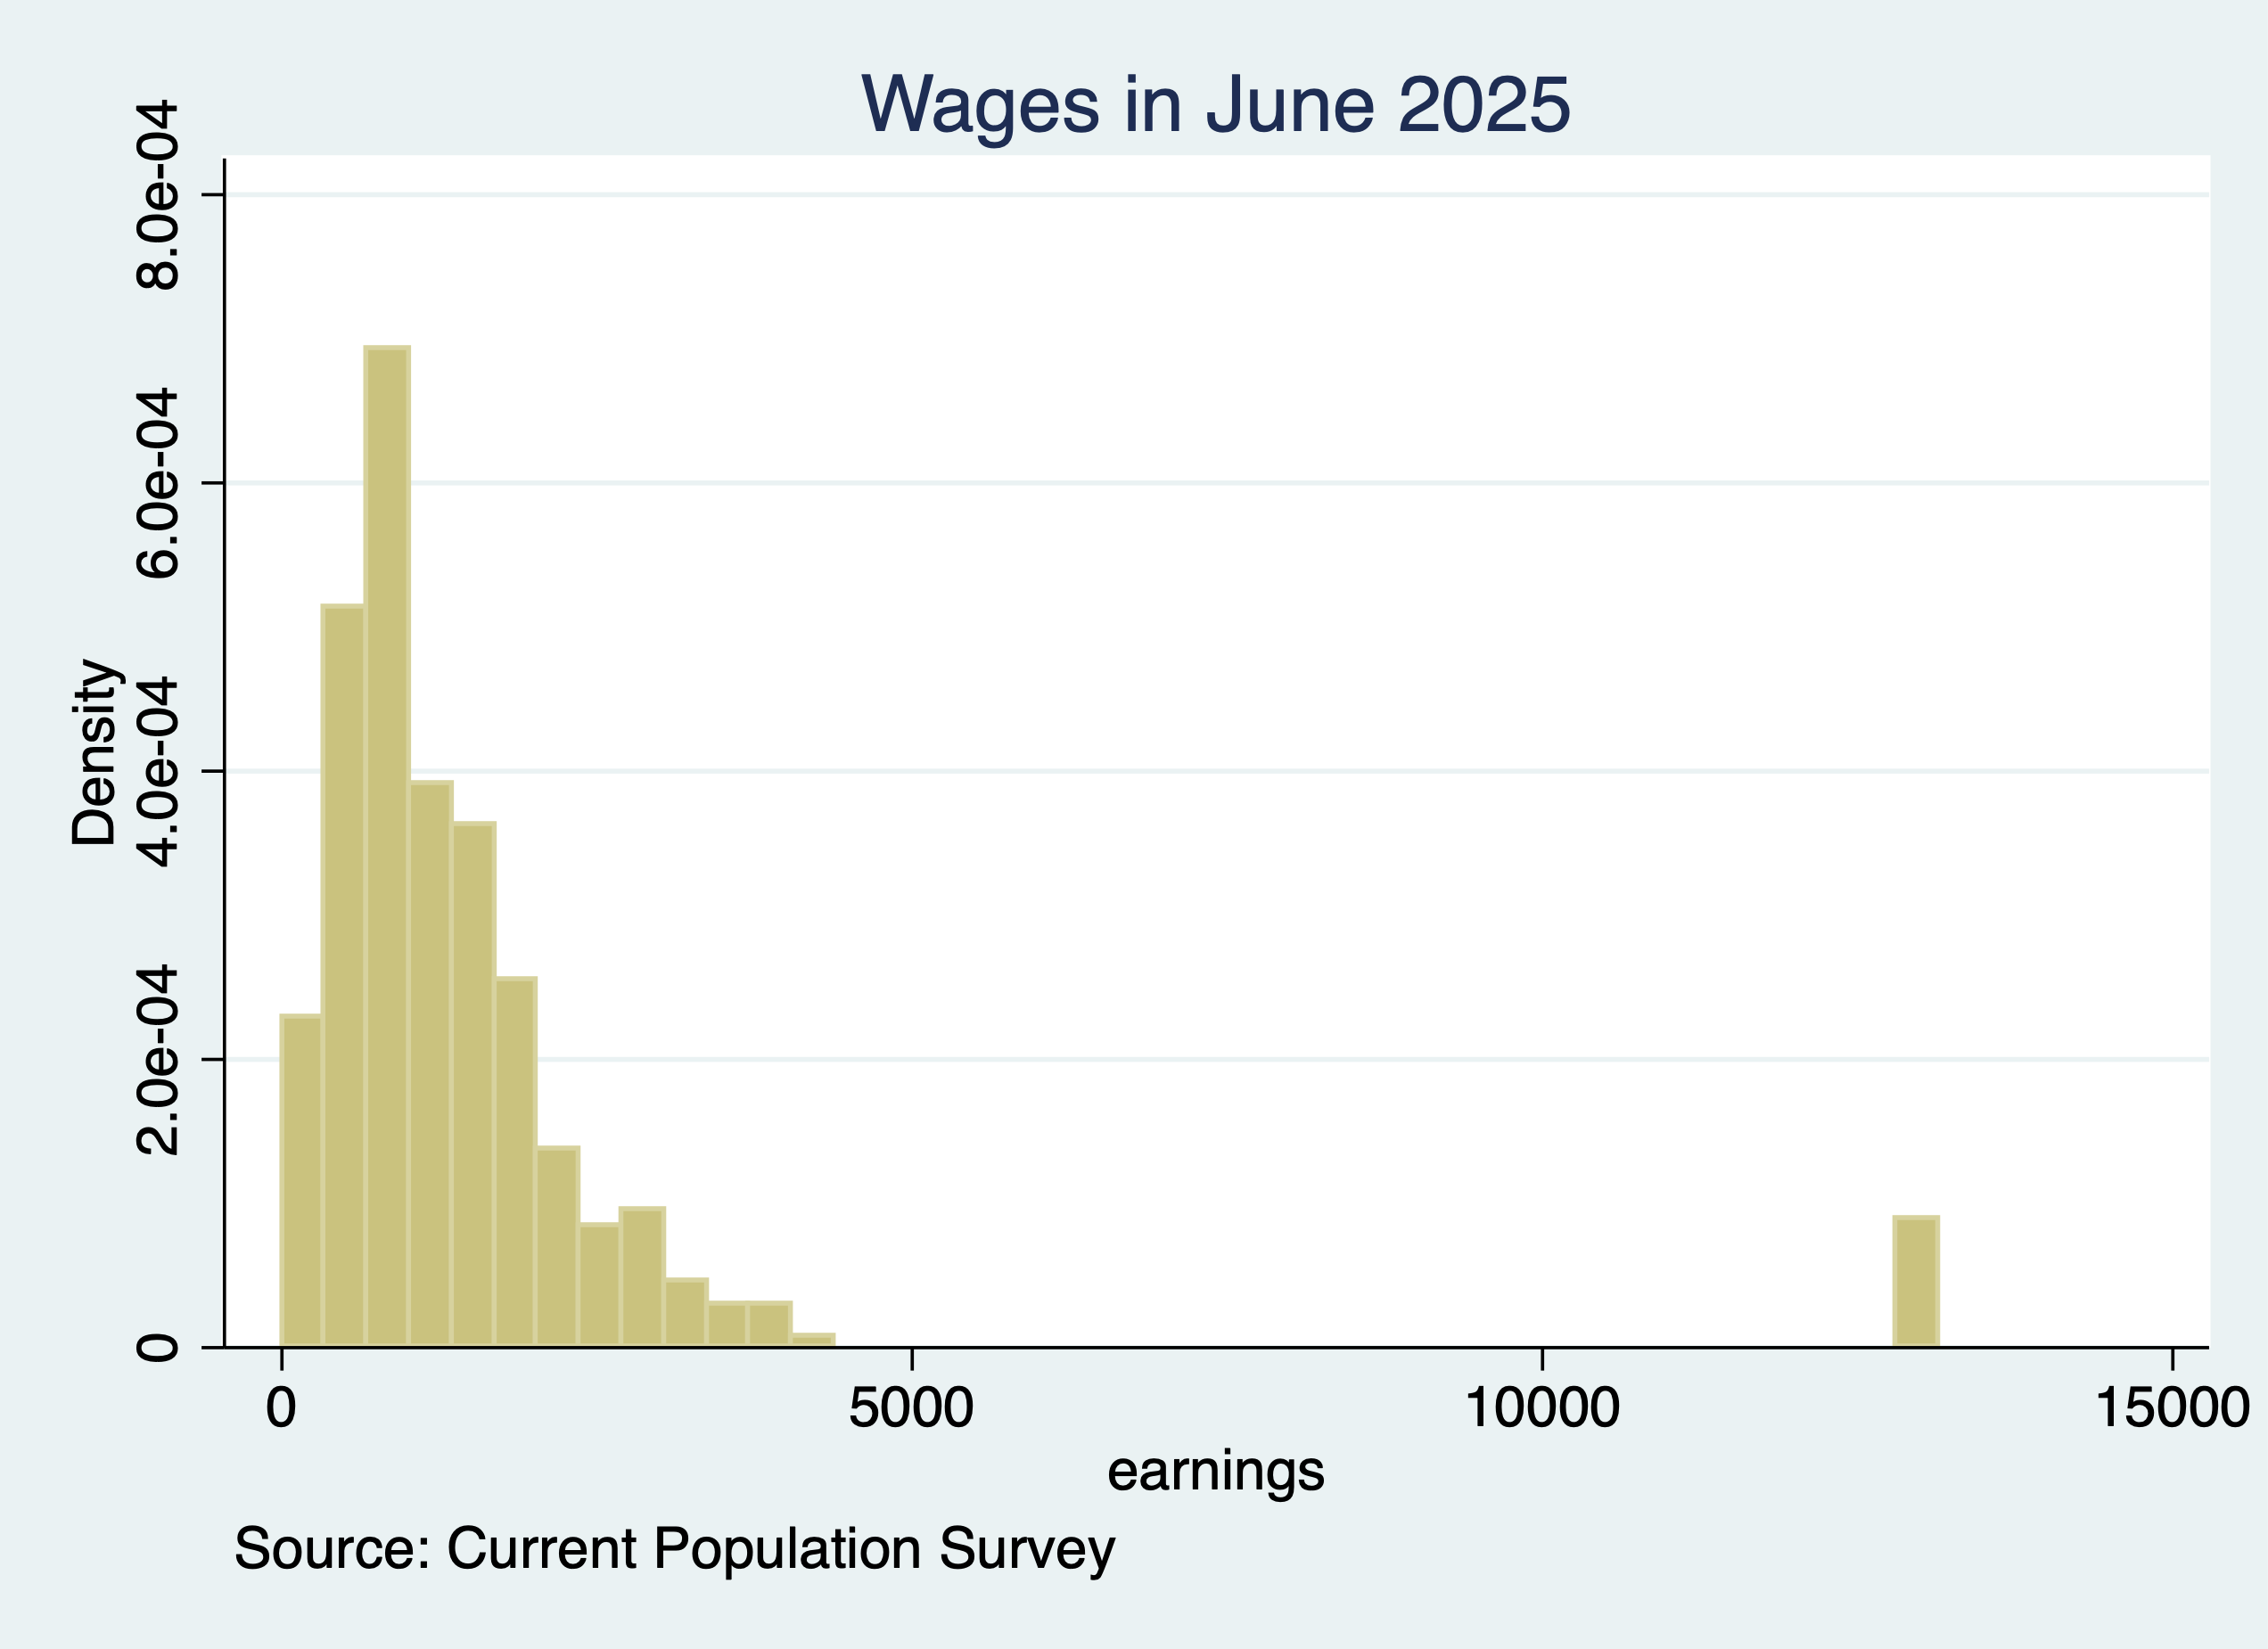
\includegraphics[keepaspectratio]{Wages_in_June_2025.png}}
\caption{Wages Histogram}
\end{figure}

\chapter{Stata Programming Techniques Helpful for Econ 645}\label{stata-programming-techniques-helpful-for-econ-645}

A brief overview of techniques that will be helpful for completing assignments and empirical project topics include - Local Macros, Loops, Tempfiles, By Sort and Egen, and Weights\textless{}

\begin{enumerate}
\def\labelenumi{\arabic{enumi}.}
\tightlist
\item
  Macros
\item
  Local Macros
\item
  Global Macros
\item
  Loops
\item
  Dataframes and Tempfiles
\item
  Appending\\
\item
  Bysort and EGEN
\item
  Survey Weights
\item
  Accessing results in Stata's stored memory
\end{enumerate}

\section{Stata Programming: Macros}\label{stata-programming-macros}

One of the essential parts of Stata programming are macros. Macros variables have many uses and can contain strings or numerics. We can use them in loops, in regressions, in calling temporary files, etc. There are two kinds of macros: local and global.

\section{Local Macros}\label{local-macros}

Local macros work within a single executed do file and removed once the session is run. If you are running local macros you must run the line of code that initializes the macro and the command that utilizes it.

You need to initialize the local macro
E.g.: local i = 1
\emph{Key}: You need to call the macro with \texttt{key\ (or\ left\ quote\ key\ just\ above\ tab\ key)\ and\ \textquotesingle{}\ key.\ E.g.:\ display\ "}i'\,''
*E.g.: replace x = 0 if y = `i'

\begin{Shaded}
\begin{Highlighting}[]
\KeywordTok{local}\NormalTok{ i = 1}
\KeywordTok{display} \StringTok{"\textasciigrave{}i\textquotesingle{}"}
\end{Highlighting}
\end{Shaded}

\begin{verbatim}
1
\end{verbatim}

\begin{Shaded}
\begin{Highlighting}[]
\KeywordTok{local} \KeywordTok{k}\NormalTok{ = }\OtherTok{\textasciigrave{}i\textquotesingle{}}\NormalTok{ + 1}
\KeywordTok{display} \StringTok{"\textasciigrave{}k\textquotesingle{}"}
\end{Highlighting}
\end{Shaded}

\begin{verbatim}
2
\end{verbatim}

\section{Global Macros}\label{global-macros}

Global macros are variables that stays within memory even after a new session is run. These macro varibles can work across multiple do files, as well. You need to initialize a global macro E.g.:

\begin{Shaded}
\begin{Highlighting}[]
\KeywordTok{global}\NormalTok{ j = 2}
\end{Highlighting}
\end{Shaded}

Next, you call the macro with \$

\begin{Shaded}
\begin{Highlighting}[]
\KeywordTok{display} \StringTok{"$j"}
\end{Highlighting}
\end{Shaded}

\begin{verbatim}
2
\end{verbatim}

You can use local and global macro variables for qualifiers, as well

\begin{Shaded}
\begin{Highlighting}[]
\KeywordTok{replace}\NormalTok{ z = 1 }\KeywordTok{if} \FunctionTok{y}\NormalTok{ = }\OtherTok{$i}
\end{Highlighting}
\end{Shaded}

Another great use of macros is to find a list of for local levels of a categorical variable, and store it in macro variable

\begin{Shaded}
\begin{Highlighting}[]
\KeywordTok{levelsof}\NormalTok{ varname, }\KeywordTok{local}\NormalTok{(}\KeywordTok{levels}\NormalTok{) }
\KeywordTok{foreach} \OtherTok{l} \KeywordTok{of} \KeywordTok{local} \KeywordTok{levels}\NormalTok{ \{}
\NormalTok{  command }\KeywordTok{if}\NormalTok{ varname == }\OtherTok{\textasciigrave{}l\textquotesingle{}}
\NormalTok{\}}
\end{Highlighting}
\end{Shaded}

We'll demo this later, but it is quite useful

You can also use local macros to test regression models
We'll demo this later, as well

\section{Looping}\label{looping}

\emph{Looping has many uses when you want to apply a function or command over
}a repeated set of values
\emph{There is forvalues and foreach - I typically use foreach given it's versatility
}but Stata says that forvalues can be more efficient
*E.g.: Loop over years and iterate i

\subsection{Loop over a number}\label{loop-over-a-number}

\begin{Shaded}
\begin{Highlighting}[]
\KeywordTok{local}\NormalTok{ i = 0}
\KeywordTok{foreach}\NormalTok{ num }\KeywordTok{of}\NormalTok{ numlist 2015/2019 \{}
  \KeywordTok{display} \StringTok{"\textasciigrave{}num\textquotesingle{}"}
  \KeywordTok{local}\NormalTok{ i = }\OtherTok{\textasciigrave{}i\textquotesingle{}}\NormalTok{+1}
  \KeywordTok{display} \StringTok{"This is the \textasciigrave{}i\textquotesingle{} loop"}
\NormalTok{\}}
\end{Highlighting}
\end{Shaded}

\begin{verbatim}
2015
This is the 1 loop
2016
This is the 2 loop
2017
This is the 3 loop
2018
This is the 4 loop
2019
This is the 5 loop
\end{verbatim}

\subsection{Loop over a local macro}\label{loop-over-a-local-macro}

*E.g.: Loop over months and years to read in new files

\begin{Shaded}
\begin{Highlighting}[]
\KeywordTok{local} \FunctionTok{month}\NormalTok{ jan feb mar apr may jun jul aug sep oct nov dec}
\KeywordTok{foreach} \FunctionTok{y} \KeywordTok{of}\NormalTok{ numlist 2018/2019 \{}
  \KeywordTok{foreach} \FunctionTok{m} \KeywordTok{of} \KeywordTok{local} \FunctionTok{month}\NormalTok{ \{}
    \KeywordTok{local}\NormalTok{ filename = }\StringTok{"\textasciigrave{}m\textquotesingle{}\textasciigrave{}y\textquotesingle{}.dta"}
    \KeywordTok{display} \StringTok{"\textasciigrave{}filename\textquotesingle{}"}
\NormalTok{  \}}
\NormalTok{\}}
\end{Highlighting}
\end{Shaded}

\begin{verbatim}
jan2018.dta
feb2018.dta
mar2018.dta
apr2018.dta
may2018.dta
jun2018.dta
jul2018.dta
aug2018.dta
sep2018.dta
oct2018.dta
nov2018.dta
dec2018.dta
jan2019.dta
feb2019.dta
mar2019.dta
apr2019.dta
may2019.dta
jun2019.dta
jul2019.dta
aug2019.dta
sep2019.dta
oct2019.dta
nov2019.dta
dec2019.dta
\end{verbatim}

\section{Data Frames and Tempfiles}\label{data-frames-and-tempfiles}

Data frames are a relatively new part of Stata (Stata 16+) that let you switch between datasets. Before you could only work on one dataset at a time. You can read an introduction to Stata data frames from
Asjad Naqvi.

For older versions of Stata, we have the tempfiles workaround. Tempfiles are useful since they are a bypass around an older Stata limitation of one dataframe at a time. Later iterations of Stata introduced the dataframe functionality, but the tempfile method still works well.
We will append three years of CPS MORG data from NBER and generate short 1-year panels. \emph{Note}: Tempfiles are really just macros.

\section{Appending multiple CPS files}\label{appending-multiple-cps-files}

Get CPS Data

Small CPS Files have only a few variables in them compared to the usual.
The full Census CPS micro data files found at:
https://www.census.gov/data/datasets/time-series/demo/cps/cps-basic.html.

Set up initial tempfile so we can add each year of CPS data. Save the macro and set it to emptyok.

\begin{Shaded}
\begin{Highlighting}[]
\KeywordTok{tempfile}\NormalTok{ cps}
\KeywordTok{save} \OtherTok{\textasciigrave{}cps\textquotesingle{}}\NormalTok{, emptyok}
\end{Highlighting}
\end{Shaded}

Create a local variable to loop over each year and month to append monthly CPS files into 1 cps file.

\begin{Shaded}
\begin{Highlighting}[]
\NormalTok{cd }\StringTok{"/Users/Sam/Desktop/Data/CPS"}
\NormalTok{*Set }\FunctionTok{month} \KeywordTok{macro}
\KeywordTok{local} \FunctionTok{month}\NormalTok{ jan feb mar apr may jun jul aug sep oct nov dec}
\KeywordTok{local}\NormalTok{ filecount = 0}

\KeywordTok{tempfile}\NormalTok{ cps}
\KeywordTok{save} \OtherTok{\textasciigrave{}cps\textquotesingle{}}\NormalTok{, emptyok}

\KeywordTok{foreach} \FunctionTok{y} \KeywordTok{of}\NormalTok{ numlist 23/24 \{}

  \KeywordTok{foreach} \FunctionTok{m} \KeywordTok{of} \KeywordTok{local} \FunctionTok{month}\NormalTok{ \{}
        
\NormalTok{    *Show the }\FunctionTok{year}\NormalTok{ and }\FunctionTok{month}
    \KeywordTok{display} \StringTok{"\textasciigrave{}m\textquotesingle{}\textasciigrave{}y\textquotesingle{}"}
    \KeywordTok{local}\NormalTok{ filename }\StringTok{"small\textasciigrave{}m\textquotesingle{}\textasciigrave{}y\textquotesingle{}pub.dta"}
    \KeywordTok{display} \StringTok{"\textasciigrave{}filename\textquotesingle{}"}
        
\NormalTok{    *Open the }\FunctionTok{monthly} \KeywordTok{data}\NormalTok{ file}
    \KeywordTok{use} \StringTok{"\textasciigrave{}filename\textquotesingle{}"}\NormalTok{, }\KeywordTok{clear}

\NormalTok{      *Append }\FunctionTok{monthly} \KeywordTok{data}\NormalTok{ file to cps }\KeywordTok{tempfile}
      \KeywordTok{quietly} \KeywordTok{append} \KeywordTok{using} \OtherTok{\textasciigrave{}cps\textquotesingle{}}

      \KeywordTok{save} \OtherTok{\textasciigrave{}cps\textquotesingle{}}\NormalTok{, }\KeywordTok{replace}
      \KeywordTok{clear}
      
\NormalTok{      *Count the number }\KeywordTok{of} \FunctionTok{monthly}\NormalTok{ files appended}
      \KeywordTok{local}\NormalTok{ filecount = }\OtherTok{\textasciigrave{}filecount\textquotesingle{}}\NormalTok{ + 1}
\NormalTok{    \}}
\NormalTok{\}}
\NormalTok{*Get the appended CPS File}
\KeywordTok{use} \OtherTok{\textasciigrave{}cps\textquotesingle{}}
\KeywordTok{tab}\NormalTok{ hrmonth hryear4}
\KeywordTok{save} \StringTok{"cps23\_24.dta"}\NormalTok{, }\KeywordTok{replace}
\end{Highlighting}
\end{Shaded}

\begin{verbatim}
/Users/Sam/Desktop/Data/CPS




(note: dataset contains 0 observations)
file /var/folders/tz/fwgb6p8923dg6yvb_kt_pw3c0000gn/T//S_36840.000001 saved

jan23
smalljan23pub.dta
file /var/folders/tz/fwgb6p8923dg6yvb_kt_pw3c0000gn/T//S_36840.000001 saved
feb23
smallfeb23pub.dta
file /var/folders/tz/fwgb6p8923dg6yvb_kt_pw3c0000gn/T//S_36840.000001 saved
mar23
smallmar23pub.dta
file /var/folders/tz/fwgb6p8923dg6yvb_kt_pw3c0000gn/T//S_36840.000001 saved
apr23
smallapr23pub.dta
file /var/folders/tz/fwgb6p8923dg6yvb_kt_pw3c0000gn/T//S_36840.000001 saved
may23
smallmay23pub.dta
file /var/folders/tz/fwgb6p8923dg6yvb_kt_pw3c0000gn/T//S_36840.000001 saved
jun23
smalljun23pub.dta
file /var/folders/tz/fwgb6p8923dg6yvb_kt_pw3c0000gn/T//S_36840.000001 saved
jul23
smalljul23pub.dta
file /var/folders/tz/fwgb6p8923dg6yvb_kt_pw3c0000gn/T//S_36840.000001 saved
aug23
smallaug23pub.dta
file /var/folders/tz/fwgb6p8923dg6yvb_kt_pw3c0000gn/T//S_36840.000001 saved
sep23
smallsep23pub.dta
file /var/folders/tz/fwgb6p8923dg6yvb_kt_pw3c0000gn/T//S_36840.000001 saved
oct23
smalloct23pub.dta
file /var/folders/tz/fwgb6p8923dg6yvb_kt_pw3c0000gn/T//S_36840.000001 saved
nov23
smallnov23pub.dta
file /var/folders/tz/fwgb6p8923dg6yvb_kt_pw3c0000gn/T//S_36840.000001 saved
dec23
smalldec23pub.dta
file /var/folders/tz/fwgb6p8923dg6yvb_kt_pw3c0000gn/T//S_36840.000001 saved
jan24
smalljan24pub.dta
file /var/folders/tz/fwgb6p8923dg6yvb_kt_pw3c0000gn/T//S_36840.000001 saved
feb24
smallfeb24pub.dta
file /var/folders/tz/fwgb6p8923dg6yvb_kt_pw3c0000gn/T//S_36840.000001 saved
mar24
smallmar24pub.dta
file /var/folders/tz/fwgb6p8923dg6yvb_kt_pw3c0000gn/T//S_36840.000001 saved
apr24
smallapr24pub.dta
file /var/folders/tz/fwgb6p8923dg6yvb_kt_pw3c0000gn/T//S_36840.000001 saved
may24
smallmay24pub.dta
file /var/folders/tz/fwgb6p8923dg6yvb_kt_pw3c0000gn/T//S_36840.000001 saved
jun24
smalljun24pub.dta
file /var/folders/tz/fwgb6p8923dg6yvb_kt_pw3c0000gn/T//S_36840.000001 saved
jul24
smalljul24pub.dta
file /var/folders/tz/fwgb6p8923dg6yvb_kt_pw3c0000gn/T//S_36840.000001 saved
aug24
smallaug24pub.dta
file /var/folders/tz/fwgb6p8923dg6yvb_kt_pw3c0000gn/T//S_36840.000001 saved
sep24
smallsep24pub.dta
file /var/folders/tz/fwgb6p8923dg6yvb_kt_pw3c0000gn/T//S_36840.000001 saved
oct24
smalloct24pub.dta
file /var/folders/tz/fwgb6p8923dg6yvb_kt_pw3c0000gn/T//S_36840.000001 saved
nov24
smallnov24pub.dta
file /var/folders/tz/fwgb6p8923dg6yvb_kt_pw3c0000gn/T//S_36840.000001 saved
dec24
smalldec24pub.dta
file /var/folders/tz/fwgb6p8923dg6yvb_kt_pw3c0000gn/T//S_36840.000001 saved

           |        HRYEAR4
   HRMONTH |      2023       2024 |     Total
-----------+----------------------+----------
         1 |   125,982    126,802 |   252,784 
         2 |   124,754    126,784 |   251,538 
         3 |   124,477    124,581 |   249,058 
         4 |   126,798    126,850 |   253,648 
         5 |   127,559    126,945 |   254,504 
         6 |   127,491    126,112 |   253,603 
         7 |   127,424    126,158 |   253,582 
         8 |   127,930    127,031 |   254,961 
         9 |   126,665    126,590 |   253,255 
        10 |   127,941    126,387 |   254,328 
        11 |   126,917    126,686 |   253,603 
        12 |   126,832    126,743 |   253,575 
-----------+----------------------+----------
     Total | 1,520,770  1,517,669 | 3,038,439 


file cps23_24.dta saved
\end{verbatim}

CPS Basic Data Dictionary can be found at:
CPS Basic Data Dictionary.

Check all years are there

\section{By Sort and EGEN}\label{by-sort-and-egen}

Please note that we will get into bysort egen later in the semester. However, bysort: egen is a powerful combination that it is worth bring up now. You can summarize, replace, or create new variables by multiple groups
with the by sort and egen commands
Let's generate laborforce

\begin{enumerate}
\def\labelenumi{\arabic{enumi}.}
\tightlist
\item
  1 is employed at work;
\item
  2 is employed absent;
\item
  3 is unemployed layoff;
\item
  4 is unemployed looking;
\item
  5 is NILF retired;
\item
  6 is NILF disabiled; and
\item
  7 is NILF other
\end{enumerate}

\begin{Shaded}
\begin{Highlighting}[]
\KeywordTok{gen}\NormalTok{ laborforce = .}
\KeywordTok{replace}\NormalTok{ laborforce = 0 }\KeywordTok{if}\NormalTok{ pemlr \textgreater{}= 5 \& pemlr \textless{}= 7}
\KeywordTok{replace}\NormalTok{ laborforce = 1 }\KeywordTok{if}\NormalTok{ pemlr \textgreater{}= 1 \& pemlr \textless{}= 4}
\KeywordTok{label} \KeywordTok{define}\NormalTok{ laborforce1 0 }\StringTok{"NILF"}\NormalTok{ 1 }\StringTok{"Labor Force"}
\KeywordTok{label} \KeywordTok{values}\NormalTok{ laborforce laborforce1}
\KeywordTok{tab}\NormalTok{ laborforce}

\KeywordTok{gen}\NormalTok{ employed = .}
\KeywordTok{replace}\NormalTok{ employed = 0 }\KeywordTok{if}\NormalTok{ pemlr \textgreater{}= 3 \& pemlr \textless{}= 7}
\KeywordTok{replace}\NormalTok{ employed = 1 }\KeywordTok{if}\NormalTok{ pemlr \textgreater{}= 1 \& pemlr \textless{}= 2}
\KeywordTok{label} \KeywordTok{define}\NormalTok{ employed1 0 }\StringTok{"Not Employed"}\NormalTok{ 1 }\StringTok{"Employed"}
\KeywordTok{label} \KeywordTok{values}\NormalTok{ employed employed1}
\KeywordTok{tab}\NormalTok{ employed}
\end{Highlighting}
\end{Shaded}

Generate a race/ethnicity category from existing

\begin{Shaded}
\begin{Highlighting}[]
\KeywordTok{gen}\NormalTok{ race\_ethnicity = .}
\KeywordTok{replace}\NormalTok{ race\_ethnicity = 1 }\KeywordTok{if}\NormalTok{ ptdtrace == 1 \& pehspnon == 2}
\KeywordTok{replace}\NormalTok{ race\_ethnicity = 2 }\KeywordTok{if}\NormalTok{ ptdtrace == 2 \& pehspnon == 2 }
\KeywordTok{replace}\NormalTok{ race\_ethnicity = 3 }\KeywordTok{if}\NormalTok{ pehspnon == 1}
\KeywordTok{replace}\NormalTok{ race\_ethnicity = 4 }\KeywordTok{if}\NormalTok{ ptdtrace == 3 \& pehspnon == 2}
\KeywordTok{replace}\NormalTok{ race\_ethnicity = 5 }\KeywordTok{if}\NormalTok{ (ptdtrace == 4 | ptdtrace == 5) \& pehspnon == 2}
\KeywordTok{replace}\NormalTok{ race\_ethnicity = 6 }\KeywordTok{if}\NormalTok{ (ptdtrace \textgreater{}= 6 \& ptdtrace \textless{}= 26) \& pehspnon == 2}
\KeywordTok{label} \KeywordTok{define}\NormalTok{ race\_ethnicity1 1 }\StringTok{"White NH"}\NormalTok{ 2 }\StringTok{"Black NH"}\NormalTok{ 3 }\StringTok{"Hispanic or Latino/a"} \CommentTok{///}
\NormalTok{4 }\StringTok{"Native American NH"}\NormalTok{ 5 }\StringTok{"Asian or Pacific Islander NH"}\NormalTok{ 6 }\StringTok{"Multiracial NH"}
\KeywordTok{label} \KeywordTok{values}\NormalTok{ race\_ethnicity race\_ethnicity1}
\KeywordTok{tab}\NormalTok{ race\_ethnicity }
\end{Highlighting}
\end{Shaded}

Sort by Sex

\begin{Shaded}
\begin{Highlighting}[]
\KeywordTok{sort}\NormalTok{ pesex}
\NormalTok{*Summarize laborforce }\KeywordTok{by}\NormalTok{ sex}
\KeywordTok{by}\NormalTok{ pesex: }\KeywordTok{sum}\NormalTok{ laborforce}
\KeywordTok{bysort}\NormalTok{: }\KeywordTok{sum}\NormalTok{ laborforce}
\end{Highlighting}
\end{Shaded}

Sort by Sex and Race.

\begin{Shaded}
\begin{Highlighting}[]
\KeywordTok{sort}\NormalTok{ pesex race\_ethnicity}
\NormalTok{*Summarize laborforce }\KeywordTok{by}\NormalTok{ sex and race}
\KeywordTok{by}\NormalTok{ pesex race\_ethnicity: }\KeywordTok{sum}\NormalTok{ laborforce}
\KeywordTok{bysort}\NormalTok{ pesex race\_ethnicity: }\KeywordTok{sum}\NormalTok{ laborforce}
\end{Highlighting}
\end{Shaded}

Generate Age Bin to find individuals over 16.

\begin{Shaded}
\begin{Highlighting}[]
\KeywordTok{gen}\NormalTok{ over\_16 = .}
\KeywordTok{replace}\NormalTok{ over\_16 = 0 }\KeywordTok{if}\NormalTok{ prtage \textless{} 16}
\KeywordTok{replace}\NormalTok{ over\_16 = 1 }\KeywordTok{if}\NormalTok{ prtage \textgreater{}= 16}
\KeywordTok{label} \KeywordTok{define}\NormalTok{ over\_16a 0 }\StringTok{"Under 16"}\NormalTok{ 1 }\StringTok{"16 and older"}
\KeywordTok{label} \KeywordTok{values}\NormalTok{ over\_16 over\_16a}
\KeywordTok{tab}\NormalTok{ over\_16}
\end{Highlighting}
\end{Shaded}

Generate unweighted laborforce participation rate for each group with by sort and egen. Bysort works, as well, but I usually use sort on one line and by on the other

\begin{Shaded}
\begin{Highlighting}[]
\KeywordTok{sort}\NormalTok{ pesex race\_ethnicity}
\KeywordTok{by}\NormalTok{ pesex race\_ethnicity: }\KeywordTok{egen}\NormalTok{ mean\_lfpr = }\KeywordTok{mean}\NormalTok{(laborforce) }\KeywordTok{if}\NormalTok{ over\_16 == 1}
\KeywordTok{by}\NormalTok{ pesex race\_ethnicity: }\KeywordTok{sum}\NormalTok{ mean\_lfpr}
\end{Highlighting}
\end{Shaded}

\begin{Shaded}
\begin{Highlighting}[]
\NormalTok{*Counting and indexing/subscripting within groups}
\KeywordTok{gen}\NormalTok{ idcount = .}
\KeywordTok{by}\NormalTok{ pesex race\_ethnicity: }\KeywordTok{replace}\NormalTok{ idcount = }\DataTypeTok{\_n}
\KeywordTok{gen}\NormalTok{ idcount2 = .}
\KeywordTok{by}\NormalTok{ pesex race\_ethnicity: }\KeywordTok{replace}\NormalTok{ idcount2 = idcount[\_N]}
\end{Highlighting}
\end{Shaded}

\section{Retrieving estimates stored in Stata's memory}\label{retrieving-estimates-stored-in-statas-memory}

Instead manually entering summary or regression results, we can use scalars in Stata's memory to retrieve the information. This reduces human error of copying and pasting.

For summary statistics we can use the \textbf{return list} command.

\begin{Shaded}
\begin{Highlighting}[]
\NormalTok{cd }\StringTok{"/Users/Sam/Desktop/Data/CPS"}
\KeywordTok{use}\NormalTok{ smalljan24pub.dta, }\KeywordTok{clear}
\KeywordTok{sum}\NormalTok{ pternwa }\KeywordTok{if}\NormalTok{ prerelg==1}

\FunctionTok{return} \OtherTok{list}

\KeywordTok{gen}\NormalTok{ demean\_earnings=pternwa{-}}\OtherTok{\textasciigrave{}r(mean)\textquotesingle{}} \KeywordTok{if}\NormalTok{ prerelg==1}
\KeywordTok{summarize}\NormalTok{ demean\_earnings}
\end{Highlighting}
\end{Shaded}

\begin{verbatim}
/Users/Sam/Desktop/Data/CPS

    Variable |        Obs        Mean    Std. Dev.       Min        Max
-------------+---------------------------------------------------------
     pternwa |     10,666    137274.8    146839.5          0    1125627


scalars:
                  r(N) =  10666
              r(sum_w) =  10666
               r(mean) =  137274.7503281455
                r(Var) =  21561833661.67427
                 r(sd) =  146839.4826389492
                r(min) =  0
                r(max) =  1125627
                r(sum) =  1464172487

(116,136 missing values generated)

    Variable |        Obs        Mean    Std. Dev.       Min        Max
-------------+---------------------------------------------------------
demean_ear~s |     10,666   -3.79e-12    146839.5  -137274.8   988352.2
\end{verbatim}

We can also grab information about a regression

\begin{Shaded}
\begin{Highlighting}[]
\NormalTok{cd }\StringTok{"/Users/Sam/Desktop/Data/CPS"}
\KeywordTok{use}\NormalTok{ smalljan24pub.dta, }\KeywordTok{clear}
\KeywordTok{gen}\NormalTok{ lnearn=}\FunctionTok{ln}\NormalTok{(pternwa) }\KeywordTok{if}\NormalTok{ prerelg==1}
\KeywordTok{gen} \FunctionTok{exp}\NormalTok{=prtage{-}16}
\KeywordTok{replace} \FunctionTok{exp}\NormalTok{=0 }\KeywordTok{if} \FunctionTok{exp}\NormalTok{=={-}1}

\KeywordTok{reg}\NormalTok{ lnearn c.exp\#\#c.}\FunctionTok{exp}\NormalTok{ i.peeduca i.peernlab }\KeywordTok{if}\NormalTok{ prerelg==1}

\KeywordTok{ereturn} \OtherTok{list}

\FunctionTok{matrix} \OtherTok{list} \FunctionTok{e}\NormalTok{(b)}

\NormalTok{*Coefficients and standard errors}
\KeywordTok{display}\NormalTok{ \_b[1.peernlab] \_se[1.peernlab]}
\end{Highlighting}
\end{Shaded}

\begin{verbatim}
/Users/Sam/Desktop/Data/CPS


(116,150 missing values generated)

(27,667 missing values generated)

(1,209 real changes made)

      Source |       SS           df       MS      Number of obs   =    10,652
-------------+----------------------------------   F(18, 10633)    =    238.75
       Model |  2310.98949        18  128.388305   Prob > F        =    0.0000
    Residual |  5717.80316    10,633  .537741292   R-squared       =    0.2878
-------------+----------------------------------   Adj R-squared   =    0.2866
       Total |  8028.79265    10,651  .753806465   Root MSE        =    .73331

------------------------------------------------------------------------------
      lnearn |      Coef.   Std. Err.      t    P>|t|     [95% Conf. Interval]
-------------+----------------------------------------------------------------
         exp |   .0654986   .0019087    34.31   0.000     .0617571    .0692401
             |
 c.exp#c.exp |  -.0010166   .0000324   -31.38   0.000    -.0010801   -.0009531
             |
     peeduca |
         32  |   .2151811   .2348611     0.92   0.360    -.2451906    .6755528
         33  |   .1297205   .2243499     0.58   0.563    -.3100474    .5694884
         34  |   .1947927   .2240222     0.87   0.385    -.2443328    .6339181
         35  |  -.0479483   .2153955    -0.22   0.824    -.4701637    .3742672
         36  |  -.1032521   .2123809    -0.49   0.627    -.5195583    .3130541
         37  |   .0602974   .2103972     0.29   0.774    -.3521206    .4727154
         38  |   .1407128   .2128599     0.66   0.509    -.2765325    .5579581
         39  |   .4391957    .203923     2.15   0.031     .0394684     .838923
         40  |   .4534936   .2043117     2.22   0.026     .0530045    .8539827
         41  |   .5707234   .2059659     2.77   0.006     .1669917     .974455
         42  |   .5189681   .2053085     2.53   0.011     .1165251    .9214112
         43  |    .914999   .2038914     4.49   0.000     .5153337    1.314664
         44  |   1.025085   .2044413     5.01   0.000     .6243415    1.425828
         45  |   1.463769   .2108507     6.94   0.000     1.050462    1.877076
         46  |     1.3309   .2076626     6.41   0.000     .9238427    1.737958
             |
  2.peernlab |  -.0496265    .024125    -2.06   0.040    -.0969159   -.0023371
       _cons |   10.07725   .2065816    48.78   0.000     9.672309    10.48219
------------------------------------------------------------------------------


scalars:
                  e(N) =  10652
               e(df_m) =  18
               e(df_r) =  10633
                  e(F) =  238.7547824846974
                 e(r2) =  .2878377352595289
               e(rmse) =  .7333084563678371
                e(mss) =  2310.989494457061
                e(rss) =  5717.803159756108
               e(r2_a) =  .2866321563292809
                 e(ll) =  -11800.89312136709
               e(ll_0) =  -13608.80112438194
               e(rank) =  19

macros:
            e(cmdline) : "regress lnearn c.exp##c.exp i.peeduca i.peernlab if prerelg==1"
              e(title) : "Linear regression"
          e(marginsok) : "XB default"
                e(vce) : "ols"
             e(depvar) : "lnearn"
                e(cmd) : "regress"
         e(properties) : "b V"
            e(predict) : "regres_p"
          e(estat_cmd) : "regress_estat"

matrices:
                  e(b) :  1 x 21
                  e(V) :  21 x 21

functions:
             e(sample)   


e(b)[1,21]
                     c.exp#        31b.         32.         33.         34.         35.         36.         37.
           exp       c.exp     peeduca     peeduca     peeduca     peeduca     peeduca     peeduca     peeduca
y1   .06549863  -.00101659           0   .21518108   .12972052   .19479266  -.04794826   -.1032521   .06029741

            38.         39.         40.         41.         42.         43.         44.         45.         46.
       peeduca     peeduca     peeduca     peeduca     peeduca     peeduca     peeduca     peeduca     peeduca
y1    .1407128   .43919568    .4534936   .57072336   .51896812   .91499896   1.0250848    1.463769   1.3309002

            1b.          2.            
      peernlab    peernlab       _cons
y1           0  -.04962649   10.077247

00
\end{verbatim}

\section{Survey Weights}\label{survey-weights}

We can use the Current Population Survey public use microdata and replicate published BLS numbers. We need to adjust our numbers with the appropriate weights in order to replicate the published numbers.

First, we need to adjust weights the weights. In the CSV files the weights need to be divided by 1000 since the documentation says implies 4 decimals.

Composite weights \emph{cmpwgt2}* are used for final BLS tabulations of labor force

\begin{Shaded}
\begin{Highlighting}[]

\KeywordTok{gen}\NormalTok{ cmpwgt2 = pwcmpwgt/10000}
\end{Highlighting}
\end{Shaded}

Outgoing Rotation Weights \emph{pworwgt} are used for earnings only person in interviews 4 and 8

\begin{Shaded}
\begin{Highlighting}[]
\KeywordTok{gen}\NormalTok{ orwgt2 = pworwgt/10000}
\end{Highlighting}
\end{Shaded}

PWSSWGT weights are used for general tabulations of sex, race, states, etc.

\begin{Shaded}
\begin{Highlighting}[]
\KeywordTok{gen}\NormalTok{ sswgt2 = pwsswgt/10000}
\end{Highlighting}
\end{Shaded}

\emph{PWVETWGT} are used to study the veteran population

\begin{Shaded}
\begin{Highlighting}[]
\KeywordTok{gen}\NormalTok{ vetwgt2 = pwvetwgt/10000}
\end{Highlighting}
\end{Shaded}

\emph{PWLWGT} are weights used to study someone over multiple CPS interviews

\begin{Shaded}
\begin{Highlighting}[]
\KeywordTok{gen}\NormalTok{ lgwgt2 = pwlgwgt/10000}
\end{Highlighting}
\end{Shaded}

If we are appending all months, we need to divide by 12 for the Basic CPS to get annual weights.

\begin{Shaded}
\begin{Highlighting}[]
    \KeywordTok{replace}\NormalTok{ cmpwgt2 = cmpwgt2/12}
\end{Highlighting}
\end{Shaded}

If we are appending all months across multiple years, we need to get a composite weight for all of the CPS files

\begin{Shaded}
\begin{Highlighting}[]
\NormalTok{cd }\StringTok{"/Users/Sam/Desktop/Data/CPS"}
\KeywordTok{use}\NormalTok{ cps23\_24.dta}
\KeywordTok{gen}\NormalTok{ cmpwgt3 = pwcmpwgt/24}
\end{Highlighting}
\end{Shaded}

Use the SvySet command to set up the survey design.

\begin{Shaded}
\begin{Highlighting}[]
    \KeywordTok{svyset}\NormalTok{ [pw=cmpwgt3]}
\end{Highlighting}
\end{Shaded}

Use the svy: command vars to utilize the survey design.

\begin{Shaded}
\begin{Highlighting}[]
    \KeywordTok{svy}\NormalTok{: }\KeywordTok{tab}\NormalTok{ employed hryear4, }\FunctionTok{count}\NormalTok{ cellwidth(20) }\KeywordTok{format}\NormalTok{(\%20.2gc)}
\end{Highlighting}
\end{Shaded}

\begin{Shaded}
\begin{Highlighting}[]
\NormalTok{cd }\StringTok{"/Users/Sam/Desktop/Data/CPS"}
\KeywordTok{use}\NormalTok{ cps23\_24.dta}
\KeywordTok{gen}\NormalTok{ cmpwgt3 = pwcmpwgt/10000}
\KeywordTok{replace}\NormalTok{ cmpwgt3 = cmpwgt3/12}
\KeywordTok{svyset}\NormalTok{ [pw=cmpwgt3]}
\KeywordTok{gen}\NormalTok{ employed = .}
\KeywordTok{replace}\NormalTok{ employed = 0 }\KeywordTok{if}\NormalTok{ pemlr \textgreater{}= 3 \& pemlr \textless{}= 7}
\KeywordTok{replace}\NormalTok{ employed = 1 }\KeywordTok{if}\NormalTok{ pemlr \textgreater{}= 1 \& pemlr \textless{}= 2}
\KeywordTok{label} \KeywordTok{define}\NormalTok{ employed1 0 }\StringTok{"Not Employed"}\NormalTok{ 1 }\StringTok{"Employed"}
\KeywordTok{label} \KeywordTok{values}\NormalTok{ employed employed1}
\KeywordTok{tab}\NormalTok{ employed}
\KeywordTok{svy}\NormalTok{: }\KeywordTok{tab}\NormalTok{ employed hryear4, }\FunctionTok{count}\NormalTok{ cellwidth(20) }\KeywordTok{format}\NormalTok{(\%20.2gc)}
\end{Highlighting}
\end{Shaded}

\begin{verbatim}
/Users/Sam/Desktop/Data/CPS


(655,995 missing values generated)

(1,946,105 real changes made)

      pweight: cmpwgt3
          VCE: linearized
  Single unit: missing
     Strata 1: <one>
         SU 1: <observations>
        FPC 1: <zero>

(3,038,439 missing values generated)

(838,080 real changes made)

(1,138,576 real changes made)

    employed |      Freq.     Percent        Cum.
-------------+-----------------------------------
Not Employed |    838,080       42.40       42.40
    Employed |  1,138,576       57.60      100.00
-------------+-----------------------------------
       Total |  1,976,656      100.00

(running tabulate on estimation sample)

Number of strata   =         1                Number of obs     =    1,976,656
Number of PSUs     = 1,976,656                Population size   =  535,513,623
                                              Design df         =    1,976,655

----------------------------------------------------------------------------
          |                             HRYEAR4                             
 employed |                 2023                  2024                 Total
----------+-----------------------------------------------------------------
 Not Empl |          105,905,668           107,225,904           213,131,572
 Employed |          161,036,522           161,345,530           322,382,051
          | 
    Total |          266,942,190           268,571,433           535,513,623
----------------------------------------------------------------------------
  Key:  weighted count

  Pearson:
    Uncorrected   chi2(1)         =   12.9838
    Design-based  F(1, 1976655)   =    9.8919     P = 0.0017
\end{verbatim}

\chapter{Displaying your results with publication-quality tables with estout and outreg}\label{displaying-your-results-with-publication-quality-tables-with-estout-and-outreg}

Stata has two suites of functions that help produce publication-quality tables: estout and outreg2. While it is easy to copy and paste tables, this is not a best practice. You want to have your Stata scripts reduce the amounts of pointing-and-clicking. Pointing-and-clicking is highly repeative and more prone to user error. It is better to avoid doing this! Using estout or outreg2 will help you in the long-run.

\section{Estout}\label{estout}

Estout and its functions are a way to produce publication-quality tables of descriptive statistics or regression results. The main function will be \emph{esttab}.

You can install estout by running the following ssc install command:
\url{http://repec.sowi.unibe.ch/stata/estout/index.html}

\begin{Shaded}
\begin{Highlighting}[]
\KeywordTok{ssc}\NormalTok{ install estout}
\end{Highlighting}
\end{Shaded}

Esttab is the main function in estout that provides publication-quality tables. The basics of esttab are the following:

\begin{Shaded}
\begin{Highlighting}[]
\NormalTok{esttab [ namelist ] [ }\KeywordTok{using}\NormalTok{ filename ] [ , options estout\_options ]}
\end{Highlighting}
\end{Shaded}

\subsection{Esttab Examples}\label{esttab-examples}

Here is an example of a simple regression output comparing two models. We use eststo to store the model and use esttab to display the results.

\begin{Shaded}
\begin{Highlighting}[]
\KeywordTok{quietly} \KeywordTok{sysuse}\NormalTok{ auto}
\NormalTok{eststo m1: }\KeywordTok{quietly} \KeywordTok{regress}\NormalTok{ price }\KeywordTok{weight}\NormalTok{ mpg}
\NormalTok{eststo m2: }\KeywordTok{quietly} \KeywordTok{regress}\NormalTok{ price }\KeywordTok{weight}\NormalTok{ mpg foreign}
\NormalTok{esttab m1 m2}
\end{Highlighting}
\end{Shaded}

\begin{verbatim}
                      (1)             (2)   
                    price           price   
--------------------------------------------
weight              1.747**         3.465***
                   (2.72)          (5.49)   

mpg                -49.51           21.85   
                  (-0.57)          (0.29)   

foreign                            3673.1***
                                   (5.37)   

_cons              1946.1         -5853.7   
                   (0.54)         (-1.73)   
--------------------------------------------
N                      74              74   
--------------------------------------------
t statistics in parentheses
* p<0.05, ** p<0.01, *** p<0.001
\end{verbatim}

We can replace t-statistics with pvalues with ``p''. Or, we can use ``se'' for standard errors, and we can use ci ``ci'' for confidence interval. We can add scalars to the model output as well. We can use ``F'' to display the overall F-statistic, ``df\_r'' for degrees of freedom, and ``rmse'' for root mean squared error. We can also use ``r2'' for R-Squared and ``ar2'' for adjusted R-Squared.

\begin{Shaded}
\begin{Highlighting}[]
\KeywordTok{quietly} \KeywordTok{sysuse}\NormalTok{ auto}
\NormalTok{eststo m1: }\KeywordTok{quietly} \KeywordTok{regress}\NormalTok{ price }\KeywordTok{weight}\NormalTok{ mpg}
\NormalTok{eststo m2: }\KeywordTok{quietly} \KeywordTok{regress}\NormalTok{ price }\KeywordTok{weight}\NormalTok{ mpg foreign}
\NormalTok{esttab m1 m2, }\KeywordTok{p}\NormalTok{ scalars(}\FunctionTok{F}\NormalTok{ df\_r rmse) r2 ar2}
\end{Highlighting}
\end{Shaded}

\begin{verbatim}
                      (1)             (2)   
                    price           price   
--------------------------------------------
weight              1.747**         3.465***
                  (0.008)         (0.000)   

mpg                -49.51           21.85   
                  (0.567)         (0.769)   

foreign                            3673.1***
                                  (0.000)   

_cons              1946.1         -5853.7   
                  (0.590)         (0.087)   
--------------------------------------------
N                      74              74   
R-sq                0.293           0.500   
adj. R-sq           0.273           0.478   
F                   14.74           23.29   
df_r                   71              70   
rmse               2514.0          2130.8   
--------------------------------------------
p-values in parentheses
* p<0.05, ** p<0.01, *** p<0.001
\end{verbatim}

With the title() option, we can add a title to the table output. We can also change the model names at the top of the columns with the mtitle() option. We can move the p-values, t-statistics, or standard errors to the right of the beta coefficients with the option ``wide''. We can also add a note with the addnote() option

\begin{Shaded}
\begin{Highlighting}[]
\KeywordTok{quietly} \KeywordTok{sysuse}\NormalTok{ auto}
\NormalTok{eststo m1: }\KeywordTok{quietly} \KeywordTok{regress}\NormalTok{ price }\KeywordTok{weight}\NormalTok{ mpg}
\NormalTok{eststo m2: }\KeywordTok{quietly} \KeywordTok{regress}\NormalTok{ price }\KeywordTok{weight}\NormalTok{ mpg foreign}
\NormalTok{esttab m1 m2, }\BaseNTok{title}\NormalTok{(}\StringTok{"Regression Analysis Example"}\NormalTok{) }\KeywordTok{p}\NormalTok{ scalars(}\FunctionTok{F}\NormalTok{ df\_r rmse) r2 ar2 mtitle(}\StringTok{"Model 1"} \StringTok{"Model 2"}\NormalTok{) }\KeywordTok{wide}
\end{Highlighting}
\end{Shaded}

\begin{verbatim}
Regression Analysis Example
----------------------------------------------------------------------
                      (1)                          (2)                
                  Model 1                      Model 2                
----------------------------------------------------------------------
weight              1.747**       (0.008)        3.465***      (0.000)
mpg                -49.51         (0.567)        21.85         (0.769)
foreign                                         3673.1***      (0.000)
_cons              1946.1         (0.590)      -5853.7         (0.087)
----------------------------------------------------------------------
N                      74                           74                
R-sq                0.293                        0.500                
adj. R-sq           0.273                        0.478                
F                   14.74                        23.29                
df_r                   71                           70                
rmse               2514.0                       2130.8                
----------------------------------------------------------------------
p-values in parentheses
* p<0.05, ** p<0.01, *** p<0.001
\end{verbatim}

\subsection{Exporting into Word, Excel, or LaTex format}\label{exporting-into-word-excel-or-latex-format}

**Do not copy and paste! Automate!*

We can use esttab with the export options to export into an RTF (Word), Excel, or LaTex format.

\subsubsection{Export into Excel format}\label{export-into-excel-format}

If you want to use your table in Excel. Don't copy and paste! Just add ``using'' after esttab and include the ``.csv'' file format to the file name

\begin{Shaded}
\begin{Highlighting}[]
\KeywordTok{sysuse}\NormalTok{ auto}
\NormalTok{eststo m1: }\KeywordTok{quietly} \KeywordTok{regress}\NormalTok{ price }\KeywordTok{weight}\NormalTok{ mpg}
\NormalTok{eststo m2: }\KeywordTok{quietly} \KeywordTok{regress}\NormalTok{ price }\KeywordTok{weight}\NormalTok{ mpg foreign}
\NormalTok{esttab m1 m2 }\KeywordTok{using}\NormalTok{ example.csv, }\BaseNTok{title}\NormalTok{(}\StringTok{"Regression Analysis Example"}\NormalTok{) }\KeywordTok{p}\NormalTok{ scalars(}\FunctionTok{F}\NormalTok{ df\_r rmse) r2 ar2 mtitle(}\StringTok{"Model 1"} \StringTok{"Model 2"}\NormalTok{)}
\end{Highlighting}
\end{Shaded}

\subsubsection{Export into Word format}\label{export-into-word-format}

If you want to add your table to a Word document, add ``using'' after esttab and include the ``.rtf'' file format to the file name.

\begin{Shaded}
\begin{Highlighting}[]
\KeywordTok{sysuse}\NormalTok{ auto}
\NormalTok{eststo m1: }\KeywordTok{quietly} \KeywordTok{regress}\NormalTok{ price }\KeywordTok{weight}\NormalTok{ mpg}
\NormalTok{eststo m2: }\KeywordTok{quietly} \KeywordTok{regress}\NormalTok{ price }\KeywordTok{weight}\NormalTok{ mpg foreign}
\NormalTok{esttab m1 m2 }\KeywordTok{using}\NormalTok{ example.rtf, }\BaseNTok{title}\NormalTok{(}\StringTok{"Regression Analysis Example"}\NormalTok{) }\KeywordTok{p}\NormalTok{ scalars(}\FunctionTok{F}\NormalTok{ df\_r rmse) r2 ar2 mtitle(}\StringTok{"Model 1"} \StringTok{"Model 2"}\NormalTok{)}
\end{Highlighting}
\end{Shaded}

\subsubsection{Export into LaTex format}\label{export-into-latex-format}

You can also export your tables into a LaTex table. You can export your file and load it directly into Overleaf.
Add ``using'' after esttab and include the ``.tex'' file format to the file name

\begin{Shaded}
\begin{Highlighting}[]
\KeywordTok{sysuse}\NormalTok{ auto}
\NormalTok{eststo m1: }\KeywordTok{quietly} \KeywordTok{regress}\NormalTok{ price }\KeywordTok{weight}\NormalTok{ mpg}
\NormalTok{eststo m2: }\KeywordTok{quietly} \KeywordTok{regress}\NormalTok{ price }\KeywordTok{weight}\NormalTok{ mpg foreign}
\NormalTok{esttab m1 m2 }\KeywordTok{using}\NormalTok{ example.tex, }\BaseNTok{title}\NormalTok{(}\StringTok{"Regression Analysis Example"}\NormalTok{) }\KeywordTok{p}\NormalTok{ scalars(}\FunctionTok{F}\NormalTok{ df\_r rmse) r2 ar2 mtitle(}\StringTok{"Model 1"} \StringTok{"Model 2"}\NormalTok{)}
\end{Highlighting}
\end{Shaded}

\section{Outreg2}\label{outreg2}

Outreg2 is another set of functions that help produce publication-quality tables. My preference is for esttab in estout, so I will provide you with a reference to get started with outreg2 if you are interested.

\url{https://www.princeton.edu/~otorres/Outreg2.pdf}

\begin{Shaded}
\begin{Highlighting}[]
\KeywordTok{ssc}\NormalTok{ install outreg2}
\end{Highlighting}
\end{Shaded}

\section{Example: Mincer Equations - Replicate Tables}\label{example-mincer-equations---replicate-tables}

\emph{Important Note:} Missing values are set to -1 in the CPS PUMS (public-use micro dataset). If you do not account for missing, you will have an incorrect analysis.

First, let's generate some mutually exclusive categories of interest.
Recategorize Female:

\begin{Shaded}
\begin{Highlighting}[]
\KeywordTok{gen}\NormalTok{ female = .}
\KeywordTok{replace}\NormalTok{ female = 0 }\KeywordTok{if}\NormalTok{ pesex == 1}
\KeywordTok{replace}\NormalTok{ female = 1 }\KeywordTok{if}\NormalTok{ pesex == 2}
\KeywordTok{label} \KeywordTok{define}\NormalTok{ female1 0 }\StringTok{"Male"}\NormalTok{ 1 }\StringTok{"Female"}
\KeywordTok{label} \KeywordTok{values}\NormalTok{ female female1}
\end{Highlighting}
\end{Shaded}

Generate Union

\begin{Shaded}
\begin{Highlighting}[]
\KeywordTok{gen} \KeywordTok{union}\NormalTok{ = .}
\KeywordTok{replace} \KeywordTok{union}\NormalTok{ = 0 }\KeywordTok{if}\NormalTok{ peernlab == 2}
\KeywordTok{replace} \KeywordTok{union}\NormalTok{ = 1 }\KeywordTok{if}\NormalTok{ peernlab == 1}
\KeywordTok{label} \KeywordTok{define}\NormalTok{ union1 0 }\StringTok{"Nonunion"}\NormalTok{ 1 }\StringTok{"Union"}
\KeywordTok{label} \KeywordTok{values} \KeywordTok{union}\NormalTok{ union1}
\end{Highlighting}
\end{Shaded}

Our outcome of interest: Weekly Earnings - \emph{PTERNWA}.
\emph{Note:} Documentation says that the data in pternwa imply 2 decimals, so we need to divide by 100. We will also use the variable PRERELG to flag individuals with valid earnings.

\begin{Shaded}
\begin{Highlighting}[]
\KeywordTok{gen}\NormalTok{ earnings = .}
\KeywordTok{replace}\NormalTok{ earnings = pternwa }\KeywordTok{if}\NormalTok{ prerelg==1}
\NormalTok{*Divide }\KeywordTok{by}\NormalTok{ 100 }\KeywordTok{for}\NormalTok{ decimals}
\KeywordTok{replace}\NormalTok{ earnings = earnings/100}
\end{Highlighting}
\end{Shaded}

Generate Educational Bins

\begin{Shaded}
\begin{Highlighting}[]
\KeywordTok{tab}\NormalTok{ peeduca}
\KeywordTok{gen}\NormalTok{ educ = .}
\NormalTok{*High School Drop Out: from Less than 1st Grade to 12th Grade No Diploma}
\KeywordTok{replace}\NormalTok{ educ = 1 }\KeywordTok{if}\NormalTok{ peeduca \textgreater{}= 31 \& peeduca \textless{}38}
\NormalTok{*Graduated High School }\KeywordTok{or}\NormalTok{ GED}
\KeywordTok{replace}\NormalTok{ educ = 2 }\KeywordTok{if}\NormalTok{ peeduca == 39}
\NormalTok{*Some College}
\KeywordTok{replace}\NormalTok{ educ = 3 }\KeywordTok{if}\NormalTok{ peeduca == 40}
\NormalTok{*AA Degree: Vocational }\KeywordTok{or}\NormalTok{ Academic}
\KeywordTok{replace}\NormalTok{ educ = 4 }\KeywordTok{if}\NormalTok{ peeduca == 41 | peeduca == 42}
\NormalTok{*Bachelor\textquotesingle{}s Degree}
\KeywordTok{replace}\NormalTok{ educ = 5 }\KeywordTok{if}\NormalTok{ peeduca == 43}
\NormalTok{*Advanced Degree: Master\textquotesingle{}s, Professional, }\KeywordTok{or}\NormalTok{ Doctorate}
\KeywordTok{replace}\NormalTok{ educ = 6 }\KeywordTok{if}\NormalTok{ peeduca \textgreater{}= 44 \& peeduca \textless{}= 46}
\KeywordTok{label} \KeywordTok{define}\NormalTok{ educ1 1 }\StringTok{"High School Dropout"}\NormalTok{ 2 }\StringTok{"High School Graduate"} \CommentTok{///}
\NormalTok{                   3 }\StringTok{"Some College"}\NormalTok{ 4 }\StringTok{"Associates (VorA) Degree"} \CommentTok{///}
\NormalTok{                           5 }\StringTok{"Bachelor\textquotesingle{}s Degree"}\NormalTok{ 6 }\StringTok{"Advanced Degree"}
\KeywordTok{label} \KeywordTok{values}\NormalTok{ educ educ1}
\end{Highlighting}
\end{Shaded}

\emph{Caveat with Generating Categorical Variables in Stata}
Don't do peeduca \textgreater= 44 without peeduca \textless= 46 since missing values are very large. So you if do peeduca \textgreater= 44 and missing educational status is ``.'', then missing observations will get categorized as an advanced degree which will be a measurement error.

Generate Potential Experience

\begin{Shaded}
\begin{Highlighting}[]
\KeywordTok{gen} \FunctionTok{exp}\NormalTok{ = prtage {-} 16}
\KeywordTok{gen}\NormalTok{ exp2 = }\FunctionTok{exp}\NormalTok{*}\FunctionTok{exp}
\end{Highlighting}
\end{Shaded}

You can use local macros for testing models

\begin{Shaded}
\begin{Highlighting}[]
\KeywordTok{local}\NormalTok{ rhs1 i.educ }\FunctionTok{exp}\NormalTok{ exp2}
\KeywordTok{local}\NormalTok{ rhs2 i.educ }\FunctionTok{exp}\NormalTok{ exp2 i.female}
\KeywordTok{local}\NormalTok{ rhs3 i.educ }\FunctionTok{exp}\NormalTok{ exp2 i.female i.}\KeywordTok{union}
\KeywordTok{local}\NormalTok{ rhs4 i.educ }\FunctionTok{exp}\NormalTok{ exp2 i.female i.}\KeywordTok{union}\NormalTok{ i.hryear4 }
\KeywordTok{local}\NormalTok{ rhs5 i.educ }\FunctionTok{exp}\NormalTok{ exp2 i.female i.}\KeywordTok{union}\NormalTok{ i.hryear4 i.peio1icd}
\NormalTok{*Add interaction between female and }\KeywordTok{union}
\KeywordTok{local}\NormalTok{ rhs6 i.educ }\FunctionTok{exp}\NormalTok{ exp2 i.female\#\#i.}\KeywordTok{union}\NormalTok{ i.hryear4 i.peio1icd}
\end{Highlighting}
\end{Shaded}

Run our regression

\begin{Shaded}
\begin{Highlighting}[]
\KeywordTok{reg}\NormalTok{ earnings }\OtherTok{\textasciigrave{}rhs1\textquotesingle{}}\NormalTok{, }\KeywordTok{robust}
\KeywordTok{reg}\NormalTok{ earnings }\OtherTok{\textasciigrave{}rhs2\textquotesingle{}}\NormalTok{, }\KeywordTok{robust}
\KeywordTok{reg}\NormalTok{ earnings }\OtherTok{\textasciigrave{}rhs3\textquotesingle{}}\NormalTok{, }\KeywordTok{robust}
\KeywordTok{reg}\NormalTok{ earnings }\OtherTok{\textasciigrave{}rhs4\textquotesingle{}}\NormalTok{, }\KeywordTok{robust}
\KeywordTok{reg}\NormalTok{ earnings }\OtherTok{\textasciigrave{}rhs5\textquotesingle{}}\NormalTok{, }\KeywordTok{robust}
\KeywordTok{reg}\NormalTok{ earnings }\OtherTok{\textasciigrave{}rhs6\textquotesingle{}}\NormalTok{, }\KeywordTok{robust}
\end{Highlighting}
\end{Shaded}

\begin{verbatim}
Linear regression                               Number of obs     =    248,811
                                                F(7, 248803)      =   11601.57
                                                Prob > F          =     0.0000
                                                R-squared         =     0.2645
                                                Root MSE          =     .72359

-------------------------------------------------------------------------------------------
                          |               Robust
               lnearnings |      Coef.   Std. Err.      t    P>|t|     [95% Conf. Interval]
--------------------------+----------------------------------------------------------------
                     educ |
    High School Graduate  |    .409167   .0061648    66.37   0.000     .3970841    .4212499
            Some College  |   .4095462   .0067562    60.62   0.000     .3963043     .422788
Associates (VorA) Degree  |   .5171878   .0069999    73.88   0.000     .5034681    .5309075
       Bachelor's Degree  |   .8685378   .0063983   135.75   0.000     .8559973    .8810782
         Advanced Degree  |   1.073213   .0069293   154.88   0.000     1.059631    1.086794
                          |
                      exp |    .062107   .0004216   147.31   0.000     .0612807    .0629333
                     exp2 |  -.0009771   7.65e-06  -127.80   0.000     -.000992   -.0009621
                    _cons |   5.518003   .0069875   789.70   0.000     5.504308    5.531699
-------------------------------------------------------------------------------------------


Linear regression                               Number of obs     =    248,811
                                                F(8, 248802)      =   12342.42
                                                Prob > F          =     0.0000
                                                R-squared         =     0.3031
                                                Root MSE          =     .70438

-------------------------------------------------------------------------------------------
                          |               Robust
               lnearnings |      Coef.   Std. Err.      t    P>|t|     [95% Conf. Interval]
--------------------------+----------------------------------------------------------------
                     educ |
    High School Graduate  |   .4156047   .0059502    69.85   0.000     .4039425    .4272668
            Some College  |   .4408511   .0065453    67.35   0.000     .4280225    .4536797
Associates (VorA) Degree  |   .5596453   .0067703    82.66   0.000     .5463758    .5729149
       Bachelor's Degree  |   .9084709   .0061978   146.58   0.000     .8963234    .9206184
         Advanced Degree  |   1.121183   .0067401   166.34   0.000     1.107973    1.134394
                          |
                      exp |   .0613624   .0004132   148.52   0.000     .0605526    .0621722
                     exp2 |  -.0009637   7.50e-06  -128.53   0.000    -.0009784    -.000949
                          |
                   female |
                  Female  |   -.333084   .0028429  -117.16   0.000     -.338656   -.3275119
                    _cons |   5.660114   .0069181   818.17   0.000     5.646555    5.673673
-------------------------------------------------------------------------------------------


Linear regression                               Number of obs     =    248,811
                                                F(9, 248801)      =   11129.25
                                                Prob > F          =     0.0000
                                                R-squared         =     0.3040
                                                Root MSE          =      .7039

-------------------------------------------------------------------------------------------
                          |               Robust
               lnearnings |      Coef.   Std. Err.      t    P>|t|     [95% Conf. Interval]
--------------------------+----------------------------------------------------------------
                     educ |
    High School Graduate  |   .4125402   .0059457    69.39   0.000     .4008868    .4241935
            Some College  |   .4372733   .0065413    66.85   0.000     .4244525    .4500942
Associates (VorA) Degree  |   .5552335   .0067633    82.09   0.000     .5419776    .5684895
       Bachelor's Degree  |   .9050996   .0061986   146.02   0.000     .8929506    .9172486
         Advanced Degree  |   1.114006   .0067622   164.74   0.000     1.100752     1.12726
                          |
                      exp |   .0609065   .0004135   147.28   0.000      .060096     .061717
                     exp2 |  -.0009571   7.50e-06  -127.69   0.000    -.0009718   -.0009424
                          |
                   female |
                  Female  |  -.3322049   .0028417  -116.91   0.000    -.3377745   -.3266354
                          |
                    union |
                   Union  |   .0886408   .0041953    21.13   0.000     .0804181    .0968635
                    _cons |   5.660998   .0069149   818.66   0.000     5.647445    5.674551
-------------------------------------------------------------------------------------------


Linear regression                               Number of obs     =    248,811
                                                F(10, 248800)     =   10030.61
                                                Prob > F          =     0.0000
                                                R-squared         =     0.3049
                                                Root MSE          =     .70345

-------------------------------------------------------------------------------------------
                          |               Robust
               lnearnings |      Coef.   Std. Err.      t    P>|t|     [95% Conf. Interval]
--------------------------+----------------------------------------------------------------
                     educ |
    High School Graduate  |   .4122138   .0059457    69.33   0.000     .4005605    .4238672
            Some College  |   .4373993   .0065415    66.86   0.000      .424578    .4502205
Associates (VorA) Degree  |   .5545629   .0067628    82.00   0.000      .541308    .5678177
       Bachelor's Degree  |   .9045909   .0061969   145.97   0.000     .8924451    .9167367
         Advanced Degree  |   1.113443   .0067577   164.77   0.000     1.100198    1.126688
                          |
                      exp |   .0609184   .0004136   147.29   0.000     .0601077    .0617291
                     exp2 |  -.0009573   7.50e-06  -127.69   0.000     -.000972   -.0009426
                          |
                   female |
                  Female  |  -.3321621   .0028397  -116.97   0.000    -.3377278   -.3265963
                          |
                    union |
                   Union  |   .0887879    .004192    21.18   0.000     .0805716    .0970041
                          |
                  hryear4 |
                    2024  |   .0501524   .0028201    17.78   0.000      .044625    .0556798
                          |
                    _cons |   5.636116   .0070549   798.90   0.000     5.622289    5.649943
-------------------------------------------------------------------------------------------


Linear regression                               Number of obs     =    248,811
                                                F(22, 248788)     =    5310.25
                                                Prob > F          =     0.0000
                                                R-squared         =     0.3349
                                                Root MSE          =     .68812

-----------------------------------------------------------------------------------------------------------------
                                                |               Robust
                                     lnearnings |      Coef.   Std. Err.      t    P>|t|     [95% Conf. Interval]
------------------------------------------------+----------------------------------------------------------------
                                           educ |
                          High School Graduate  |   .3840322   .0059144    64.93   0.000     .3724401    .3956243
                                  Some College  |   .4091063   .0065253    62.70   0.000      .396317    .4218957
                      Associates (VorA) Degree  |   .5233398   .0068026    76.93   0.000      .510007    .5366727
                             Bachelor's Degree  |   .8481448   .0063508   133.55   0.000     .8356973    .8605923
                               Advanced Degree  |     1.0828   .0069954   154.79   0.000     1.069089     1.09651
                                                |
                                            exp |   .0550617   .0004126   133.46   0.000      .054253    .0558703
                                           exp2 |  -.0008699   7.42e-06  -117.31   0.000    -.0008844   -.0008553
                                                |
                                         female |
                                        Female  |  -.2669904   .0030367   -87.92   0.000    -.2729423   -.2610385
                                                |
                                          union |
                                         Union  |   .1018213   .0042456    23.98   0.000     .0934999    .1101426
                                                |
                                        hryear4 |
                                          2024  |   .0511416   .0027589    18.54   0.000     .0457342    .0565491
                                                |
                                       prmjind1 |
                              NAICS 21: Mining  |   .4601445   .0215585    21.34   0.000     .4178905    .5023985
                        NAICS 23: Construction  |   .2414286   .0139472    17.31   0.000     .2140925    .2687648
                    NAICS 31-33: Manufacturing  |   .2237477   .0137168    16.31   0.000     .1968631    .2506322
            NAICS 42,44-45: Wholesale & Retail  |  -.0344484   .0137914    -2.50   0.012    -.0614792   -.0074177
    NAICS 22,48-49: Utilities & Transportation  |   .1267323   .0143908     8.81   0.000     .0985266    .1549379
                         NAICS 51: Information  |   .2449216   .0178831    13.70   0.000     .2098712     .279972
             NAICS 52-53: Financial Activities  |   .2939349   .0142959    20.56   0.000     .2659154    .3219545
NAICS 53,55,56: Professional & Business Serv..  |   .2228786   .0138884    16.05   0.000     .1956577    .2500995
               NAICS 61-62: Education & Health  |  -.0262834   .0136592    -1.92   0.054     -.053055    .0004882
            NAICS 71-72: Leisure & Hospitality  |  -.1961534   .0141092   -13.90   0.000     -.223807   -.1684998
                      NAICS 81: Other Services  |  -.1098199    .015223    -7.21   0.000    -.1396565   -.0799833
               NAICS 92: Public Administration  |   .1422022   .0142532     9.98   0.000     .1142663    .1701381
                                                |
                                          _cons |   5.638847   .0146119   385.91   0.000     5.610208    5.667486
-----------------------------------------------------------------------------------------------------------------


Linear regression                               Number of obs     =    248,811
                                                F(23, 248787)     =    5081.12
                                                Prob > F          =     0.0000
                                                R-squared         =     0.3349
                                                Root MSE          =     .68812

-----------------------------------------------------------------------------------------------------------------
                                                |               Robust
                                     lnearnings |      Coef.   Std. Err.      t    P>|t|     [95% Conf. Interval]
------------------------------------------------+----------------------------------------------------------------
                                           educ |
                          High School Graduate  |   .3841487   .0059155    64.94   0.000     .3725543     .395743
                                  Some College  |   .4092612   .0065272    62.70   0.000      .396468    .4220543
                      Associates (VorA) Degree  |   .5235541   .0068043    76.94   0.000     .5102179    .5368903
                             Bachelor's Degree  |   .8481453   .0063508   133.55   0.000     .8356979    .8605928
                               Advanced Degree  |    1.08265    .006998   154.71   0.000     1.068934    1.096366
                                                |
                                            exp |   .0550613   .0004126   133.46   0.000     .0542527    .0558699
                                           exp2 |  -.0008699   7.42e-06  -117.31   0.000    -.0008844   -.0008554
                                                |
                                         female |
                                        Female  |  -.2680058   .0031915   -83.97   0.000    -.2742611   -.2617506
                                                |
                                          union |
                                         Union  |   .0964584   .0056709    17.01   0.000     .0853436    .1075732
                                                |
                                   female#union |
                                  Female#Union  |   .0112795    .008181     1.38   0.168     -.004755    .0273139
                                                |
                                        hryear4 |
                                          2024  |   .0511369   .0027589    18.53   0.000     .0457294    .0565443
                                                |
                                       prmjind1 |
                              NAICS 21: Mining  |   .4602906   .0215562    21.35   0.000      .418041    .5025401
                        NAICS 23: Construction  |   .2417802   .0139496    17.33   0.000     .2144393    .2691211
                    NAICS 31-33: Manufacturing  |   .2239984   .0137179    16.33   0.000     .1971116    .2508852
            NAICS 42,44-45: Wholesale & Retail  |  -.0342786    .013792    -2.49   0.013    -.0613106   -.0072466
    NAICS 22,48-49: Utilities & Transportation  |   .1272795   .0143997     8.84   0.000     .0990564    .1555026
                         NAICS 51: Information  |   .2452513   .0178858    13.71   0.000     .2101957    .2803069
             NAICS 52-53: Financial Activities  |   .2942334   .0142996    20.58   0.000     .2662066    .3222603
NAICS 53,55,56: Professional & Business Serv..  |   .2231206   .0138903    16.06   0.000     .1958961    .2503451
               NAICS 61-62: Education & Health  |    -.02622   .0136591    -1.92   0.055    -.0529915    .0005516
            NAICS 71-72: Leisure & Hospitality  |  -.1959203   .0141108   -13.88   0.000    -.2235772   -.1682635
                      NAICS 81: Other Services  |  -.1095106    .015225    -7.19   0.000    -.1393512     -.07967
               NAICS 92: Public Administration  |   .1426441   .0142568    10.01   0.000     .1147012    .1705869
                                                |
                                          _cons |   5.639084   .0146121   385.92   0.000     5.610445    5.667723
-----------------------------------------------------------------------------------------------------------------
\end{verbatim}

Use esttab for formatted results:
esttab documentation.

\begin{Shaded}
\begin{Highlighting}[]
\KeywordTok{local}\NormalTok{ rhs4 i.educ }\FunctionTok{exp}\NormalTok{ exp2 i.female i.}\KeywordTok{union}\NormalTok{ i.hryear4 }
\KeywordTok{local}\NormalTok{ rhs5 i.educ }\FunctionTok{exp}\NormalTok{ exp2 i.female i.}\KeywordTok{union}\NormalTok{ i.hryear4 i.peio1icd}
\NormalTok{*Add interaction between female and }\KeywordTok{union}
\KeywordTok{local}\NormalTok{ rhs6 i.educ }\FunctionTok{exp}\NormalTok{ exp2 i.female\#\#i.}\KeywordTok{union}\NormalTok{ i.hryear4 i.peio1icd}
\end{Highlighting}
\end{Shaded}

Use est clear to clear out your prior estimates.

\begin{Shaded}
\begin{Highlighting}[]
\KeywordTok{est} \KeywordTok{clear}
\end{Highlighting}
\end{Shaded}

We use eststo to save a model to compare it to another.

\begin{Shaded}
\begin{Highlighting}[]
\NormalTok{eststo reg1: }\KeywordTok{reg}\NormalTok{ earnings }\OtherTok{\textasciigrave{}rhs4\textquotesingle{}}
\NormalTok{eststo reg2: }\KeywordTok{reg}\NormalTok{ earnings }\OtherTok{\textasciigrave{}rhs5\textquotesingle{}}
\NormalTok{eststo }\KeywordTok{reg3}\NormalTok{: }\KeywordTok{reg}\NormalTok{ earnings }\OtherTok{\textasciigrave{}rhs6\textquotesingle{}}
\end{Highlighting}
\end{Shaded}

Output the results

\begin{Shaded}
\begin{Highlighting}[]
\NormalTok{esttab, }\BaseNTok{title}\NormalTok{ (Mincer Equation) r2 se }\KeywordTok{noconstant} \KeywordTok{star}\NormalTok{(* .10 ** .05 *** .01) }\CommentTok{///}
\NormalTok{b(\%10.3f) }\KeywordTok{drop}\NormalTok{ (*peio1icd) }\KeywordTok{wide} \KeywordTok{label}\NormalTok{.}
\end{Highlighting}
\end{Shaded}

\begin{verbatim}
Mincer Equation
-------------------------------------------------------------------------------------
                       (1)                    (2)                    (3)             
                      OLS1                   OLS2                   OLS3             
-------------------------------------------------------------------------------------
High School Gr~e     0.412***   (0.006)     0.384***   (0.006)     0.384***   (0.006)
Some College         0.437***   (0.007)     0.409***   (0.007)     0.409***   (0.007)
Associates (Vo~e     0.555***   (0.007)     0.523***   (0.007)     0.524***   (0.007)
Bachelor's Deg~e     0.905***   (0.006)     0.848***   (0.006)     0.848***   (0.006)
Advanced Degree      1.113***   (0.007)     1.083***   (0.007)     1.083***   (0.007)
exp                  0.061***   (0.000)     0.055***   (0.000)     0.055***   (0.000)
exp2                -0.001***   (0.000)    -0.001***   (0.000)    -0.001***   (0.000)
Female              -0.332***   (0.003)    -0.267***   (0.003)    -0.268***   (0.003)
Union                0.089***   (0.005)     0.102***   (0.005)     0.096***   (0.007)
HRYEAR4=2024         0.050***   (0.003)     0.051***   (0.003)     0.051***   (0.003)
NAICS 11: Agri~e                            0.000          (.)     0.000          (.)
NAICS 21: Mining                            0.460***   (0.022)     0.460***   (0.022)
NAICS 23: Cons~n                            0.241***   (0.014)     0.242***   (0.014)
NAICS 31-33: M~g                            0.224***   (0.014)     0.224***   (0.014)
NAICS 42,44-45~a                           -0.034**    (0.014)    -0.034**    (0.014)
NAICS 22,48-49~n                            0.127***   (0.015)     0.127***   (0.015)
NAICS 51: Info~n                            0.245***   (0.017)     0.245***   (0.017)
NAICS 52-53: F~e                            0.294***   (0.014)     0.294***   (0.014)
NAICS 53,55,56~B                            0.223***   (0.014)     0.223***   (0.014)
NAICS 61-62: E~h                           -0.026*     (0.014)    -0.026*     (0.014)
NAICS 71-72: L~i                           -0.196***   (0.014)    -0.196***   (0.014)
NAICS 81: Othe~s                           -0.110***   (0.015)    -0.110***   (0.015)
NAICS 92: Publ~n                            0.142***   (0.015)     0.143***   (0.015)
Female # Union                                                     0.011      (0.009)
Constant             5.636***   (0.007)     5.639***   (0.015)     5.639***   (0.015)
-------------------------------------------------------------------------------------
Observations        248811                 248811                 248811             
R-squared            0.305                  0.335                  0.335             
-------------------------------------------------------------------------------------
Standard errors in parentheses
* p<.10, ** p<.05, *** p<.01
\end{verbatim}

Estout. (2025). \emph{Making Regression Tables in Stata}. Retrieved from: \url{https://repec.sowi.unibe.ch/stata/estout/}

Mitchell, N.M. (2020). \emph{Data Management Using Stata: A Practical Handbook}. (2nd ed.). Stata Press.

UCLA Advanced Research Computing. (2025). \emph{How can I access information stored after I run a command in Stata.} Retrieved from \url{https://stats.oarc.ucla.edu/stata/faq/how-can-i-access-information-stored-after-i-run-a-command-in-stata-returned-results/}

Wooldridge (2009). \emph{Introductory Econometrics: A Modern Approach}. (4th ed.). South-Western Cengage Learning.

\bibliography{book.bib,packages.bib}

\end{document}
